\documentclass[fleqn,final]{beamer}
\mode<presentation>
{  \usetheme{I6dv} }
\usepackage{times}
\usepackage{etex}
\usepackage{amsmath,amssymb}
%\usepackage{sfmath} % for sans serif math fonts; wget http://dtrx.de/od/tex/sfmath.sty
\usepackage[english]{babel}
\usepackage[ansinew]{inputenc}
\usepackage[orientation=portrait,size=a0,scale=1.25,debug]{beamerposter}
\usepackage{booktabs,array}
\usepackage{listings}
%\usepackage{picins,graphicx}
\usepackage{xspace}
\usepackage{fp}
\usepackage{ifthen}
\usepackage[T1]{fontenc}

\usepackage{graphicx}
\usepackage{tikz,colortbl,pgf,pgfarrows,pgfnodes,pgfautomata,pgfheaps,pgfshade,eurosym, dsfont}
\listfiles
\newcommand*{\signstream}{SignStream\texttrademark\xspace}
\newcommand{\WichtigFarbe}{\color{red}}%
\newcommand{\TextFarbe}{\color{black}}%
\newcommand{\Pheight}{\rule[-5mm]{0cm}{1cm}}

\definecolor{darkblue}{rgb}{0.28,0,0.60}
\definecolor{hblue}{rgb}{0.70,0.7,1}
\definecolor{NR0}{rgb}{1,1,1}
\definecolor{NR1}{rgb}{1,1,0.8}
\definecolor{NR2}{rgb}{1,1,0.5}
\definecolor{NR3}{rgb}{1,1,0.25}
\definecolor{NR4}{rgb}{1,1,0.0}
\definecolor{NR5}{rgb}{1,0.75,0.0}
\definecolor{NR6}{rgb}{1,0.5,0.0}
\definecolor{NR7}{rgb}{1,0.25,0.0}
\definecolor{NR8}{rgb}{1,0,0.0}

\setbeamertemplate{navigation symbols}{}
\setbeamerfont{title}{series=\bfseries}
%\setbeamercolor{frametitle}{fg=UTblue}
\setbeamerfont{frametitle}{series=\bfseries}
\setbeamertemplate{frametitle}
{
\begin{centering}
\insertframetitle\vspace*{-4mm}\par
\end{centering}
}

\newcommand{\convD}{\stackrel{\text{d}}{\longrightarrow}}
\newcommand{\E}{\text{E}\,}
\newcommand{\var}{\text{V}\,}

\title{\huge Performance of Empirical Best Predictor in Informative Samples - A Monte Carlo Simulation}
\author{\large Felix Skarke, Enno Tammena, Christian Koopmann}
\institute{Freie Universit{\"a}t Berlin, Humboldt Universit{\"a}t zu Berlin}

\date{today}
\begin{document}

\begin{frame}

%
%------------------------------------------------------ ------------------------------------------------------
%
\small
\begin{columns}[t] % Wechsel in die Spaltenumgebung

\begin{column}{.3\linewidth} 
\begin{block}{Erkl�rung Vorgehen  \Pheight}
\begin{enumerate} % f�r Stichpunkte
\item Das Thema ist besonders relevant, weil ...
\item Au�erdem ...
\item Weiterhin ...

\end{enumerate}

\end{block}
\end{column}

%
%------------------------------------------------------ ------------------------------------------------------
%

\begin{column}{.3\linewidth}
\begin{block}{�bersicht Genetic Matching Algorithmus\Pheight}


\end{block}
\end{column}

%
%------------------------------------------------------ ------------------------------------------------------
%

\begin{column}{.3\linewidth}
 \begin{block}{Genetic Matching Theorie \Pheight}

\end{block}
\end{column}

%
%------------------------------------------------------ ------------------------------------------------------
%

\end{columns}


\begin{columns}[t]


%
%------------------------------------------------------ ------------------------------------------------------
%


  
\begin{column}{.3\linewidth}
    
    


    \begin{block}{Theorie \Pheight}

Formeln macht man so:
$$\int_{a}^{b} f(x)\, dx \approx (b-a)\frac{f(a) + f(b)}{2}$$


\end{block}
\end{column}


%
%------------------------------------------------------ ------------------------------------------------------
% Folie 5
   
\begin{column}{.3\linewidth}

 \begin{block}{Umsetzung \Pheight}

Hier wird das Vorgehen erkl�rt:
\begin{itemize}
\item ...
\item ...
\item ...
\end{itemize}
\end{block}
\end{column}     



%
%------------------------------------------------------ ------------------------------------------------------
% Folie 6 

  % 


\begin{column}{.3\linewidth}


\begin{block}{Implementation \Pheight}
\begin{itemize}
\item Dataset: EUSILC Data as provided by the emdi package
\item to achieve a sufficient population size $N$, randomly dublicate observations between 1 and 8 times
\item add $\varepsilon$ to the dependent variable of duplicated observations
\item take a random sample of $g$ observations from 5 income groups to get a sample of size $n$
\item calculate $frequency weights = N_{SMA,income group}/n_{SMA}/5 $
\item take random sample of $c$ observations for second level EBP data 
 
\item for 1:s \{
\begin{enumerate}  % F�r Aufz�hlungen
\item split population by SMA, take a sample of $n_{sma} / 5$ from each income group
\item estimate $Gini_{direct}, Gini_{weighted}$
\item estimate $Gini_{EBP}$  based on $l$ pseudo-populations
\item estimate $MSE_{Gini_{EBP}}$ based on $b$ bootstraps
\item expand the sample by frequency weights
\item estimate $Gini_{weighted EBP}$  based on $l$ pseudo-populations
\item save the results per SMA
\end{enumerate}
\}
 
\item calculate quality measures per SMA 
 \end{itemize}
Parameters: $N=112644, s=250, \varepsilon \sim N(0,5000), g=2000, n=10000, c=25000, l=50, b=10, SMA=District$
\end{block}



\end{column}


%
%------------------------------------------------------ ------------------------------------------------------
%
  
\end{columns}  



\begin{columns}[t]

%
%------------------------------------------------------ ------------------------------------------------------
% 10 


\begin{column}{.3\linewidth}

\begin{block}{RMSE of weighted and unweighted EBP per Domain \Pheight}
\begin{center}
	\begin{figure}
		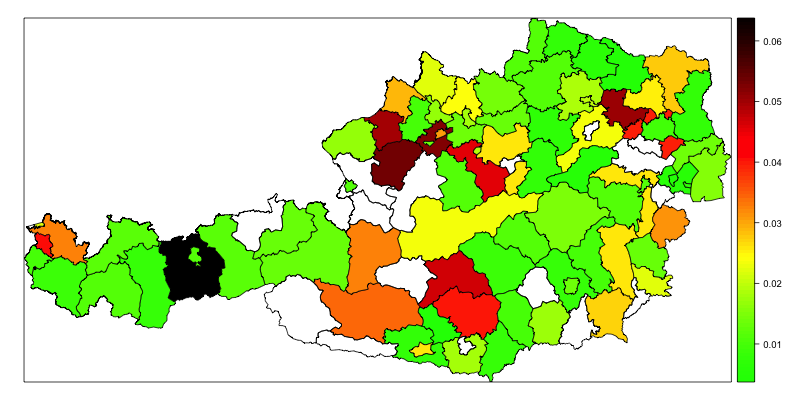
\includegraphics[width=0.9\textwidth]{EBPWeightedRMSE}
		\caption{RMSE of Weighted EBP per Domain}
	\end{figure}
		\begin{figure}
		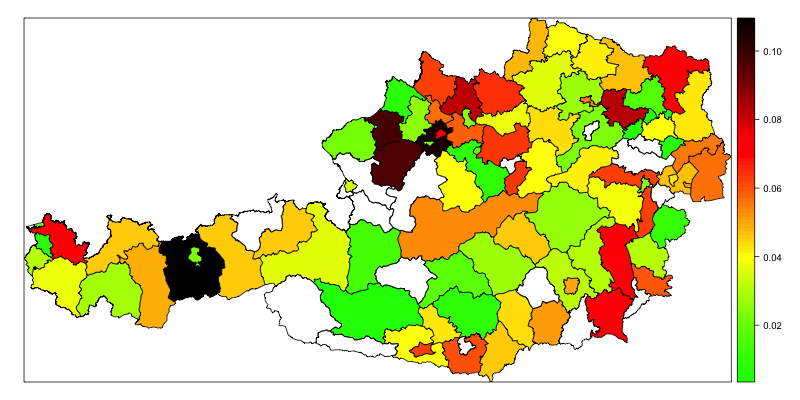
\includegraphics[width=0.9\textwidth]{EBPUnweightedRMSE}
		\caption{RMSE of Unweighted EBP per Domain}
	\end{figure}
\end{center}

\end{block}

\end{column}

%
%------------------------------------------------------ ------------------------------------------------------
% 11

\begin{column}{.3\linewidth}

\begin{block}{Domain Level MRE and RMSE of Estimators \Pheight}
\begin{center}
	\begin{figure}
		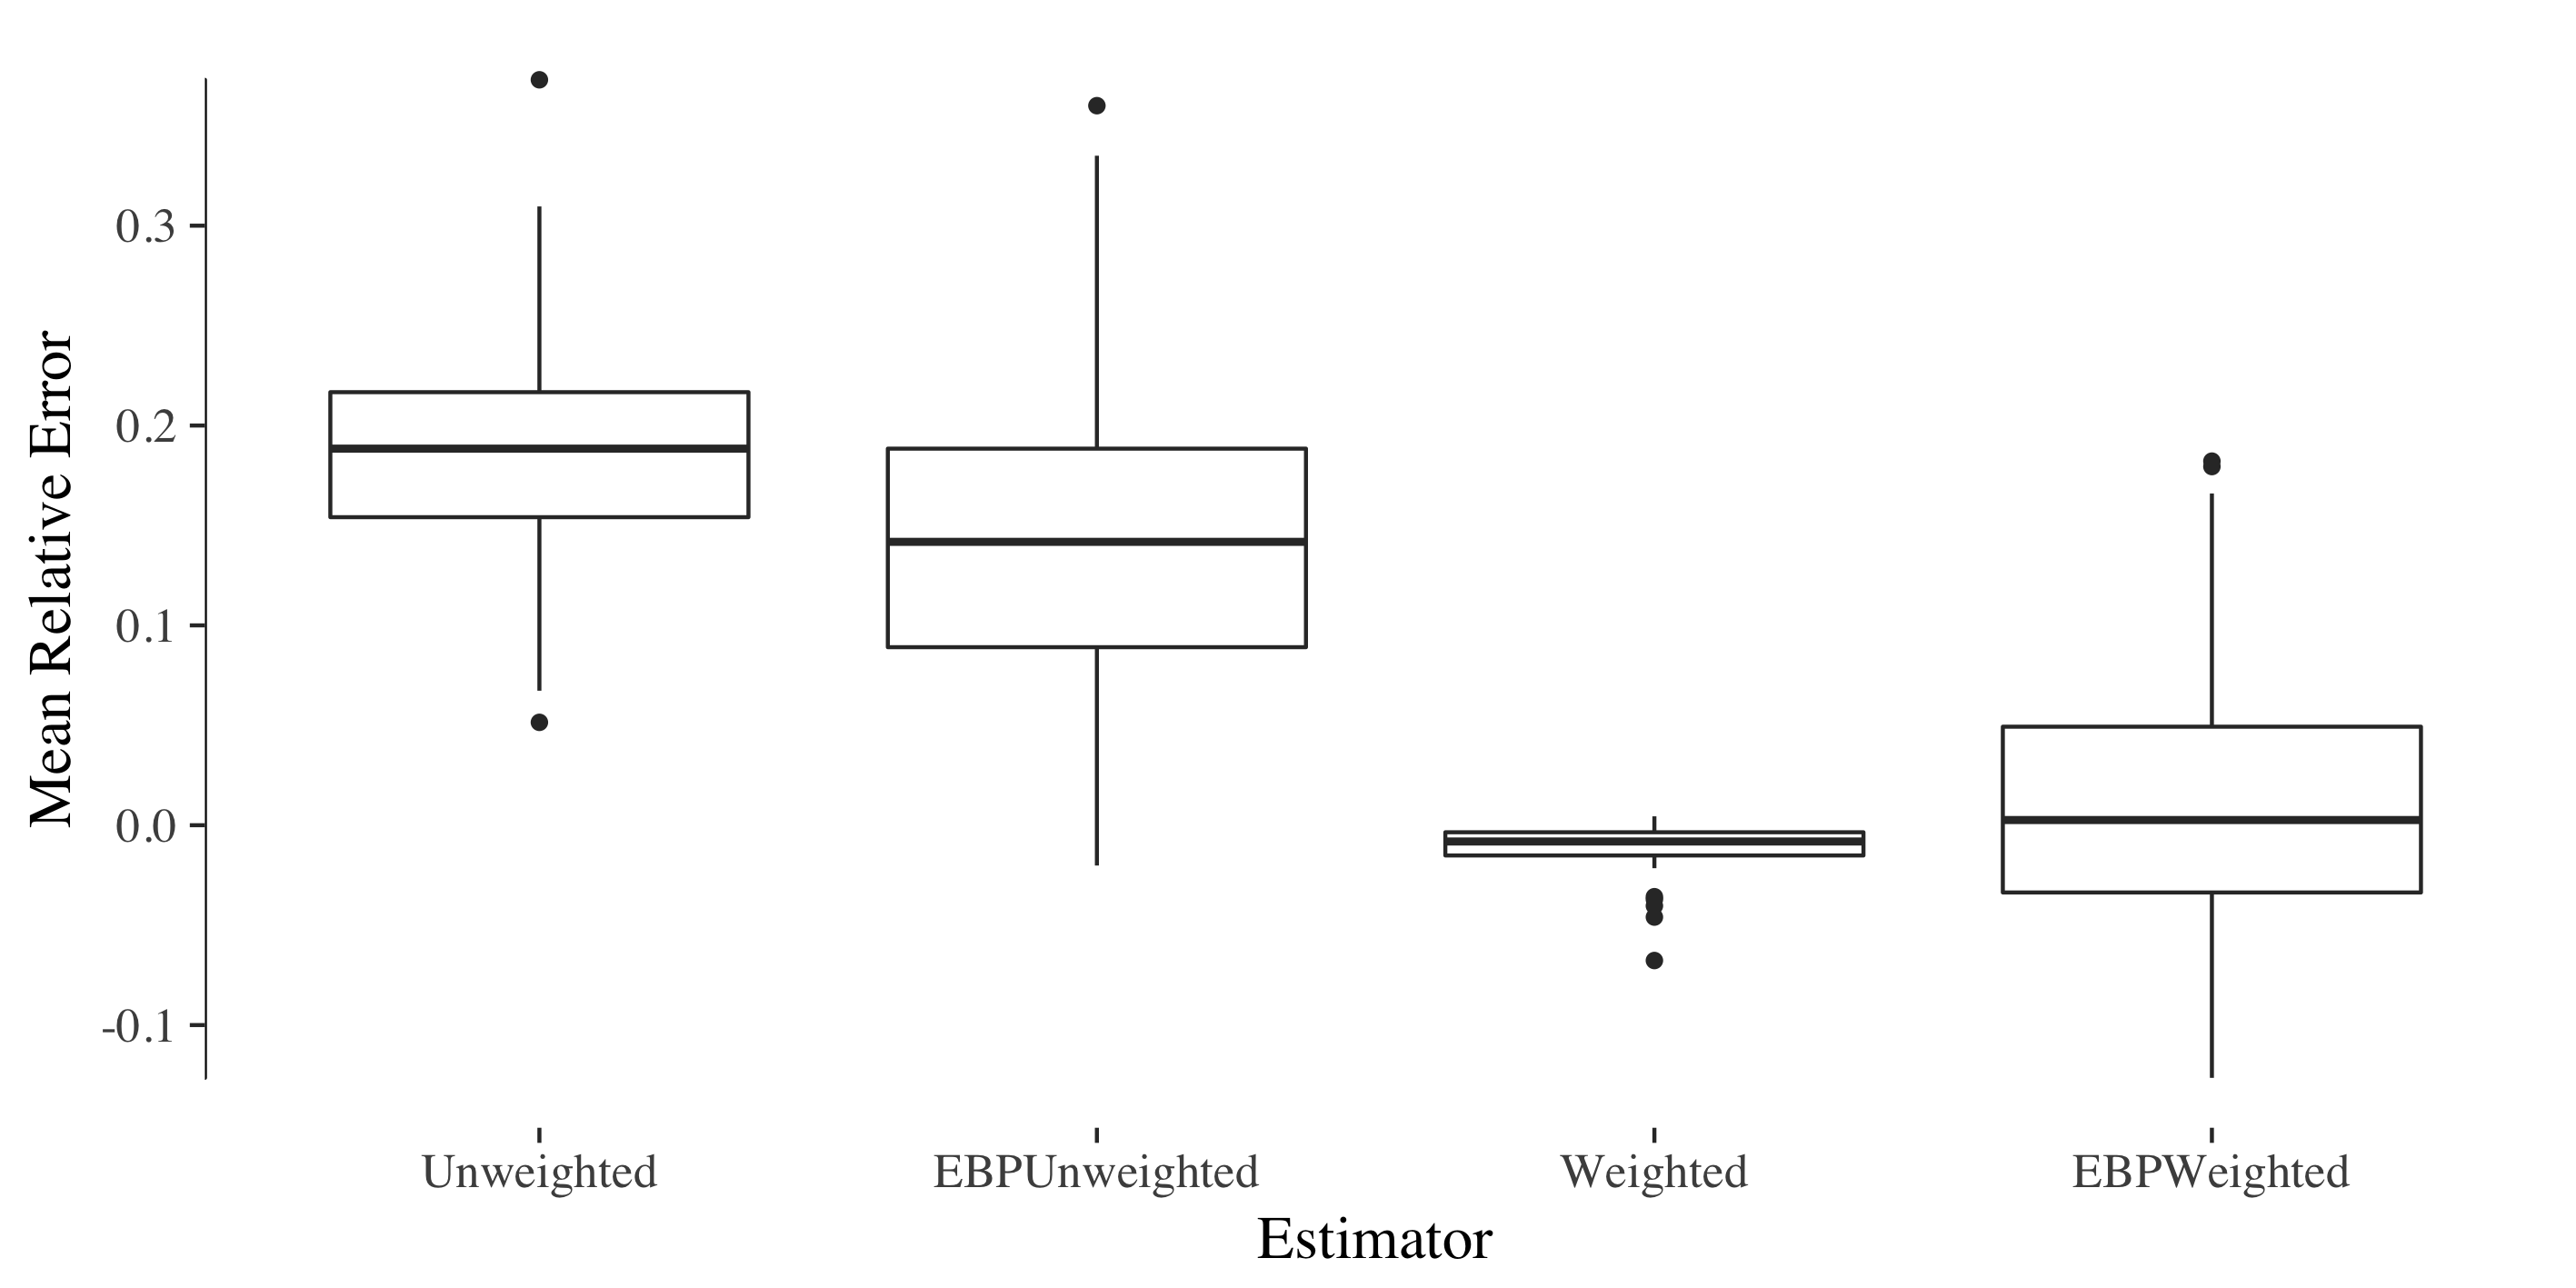
\includegraphics[width=0.9\textwidth]{BoxPlotMREByDomain}
		\caption{Boxplot of Mean Relative Error on Domain Level}
	\end{figure}
		\begin{figure}
		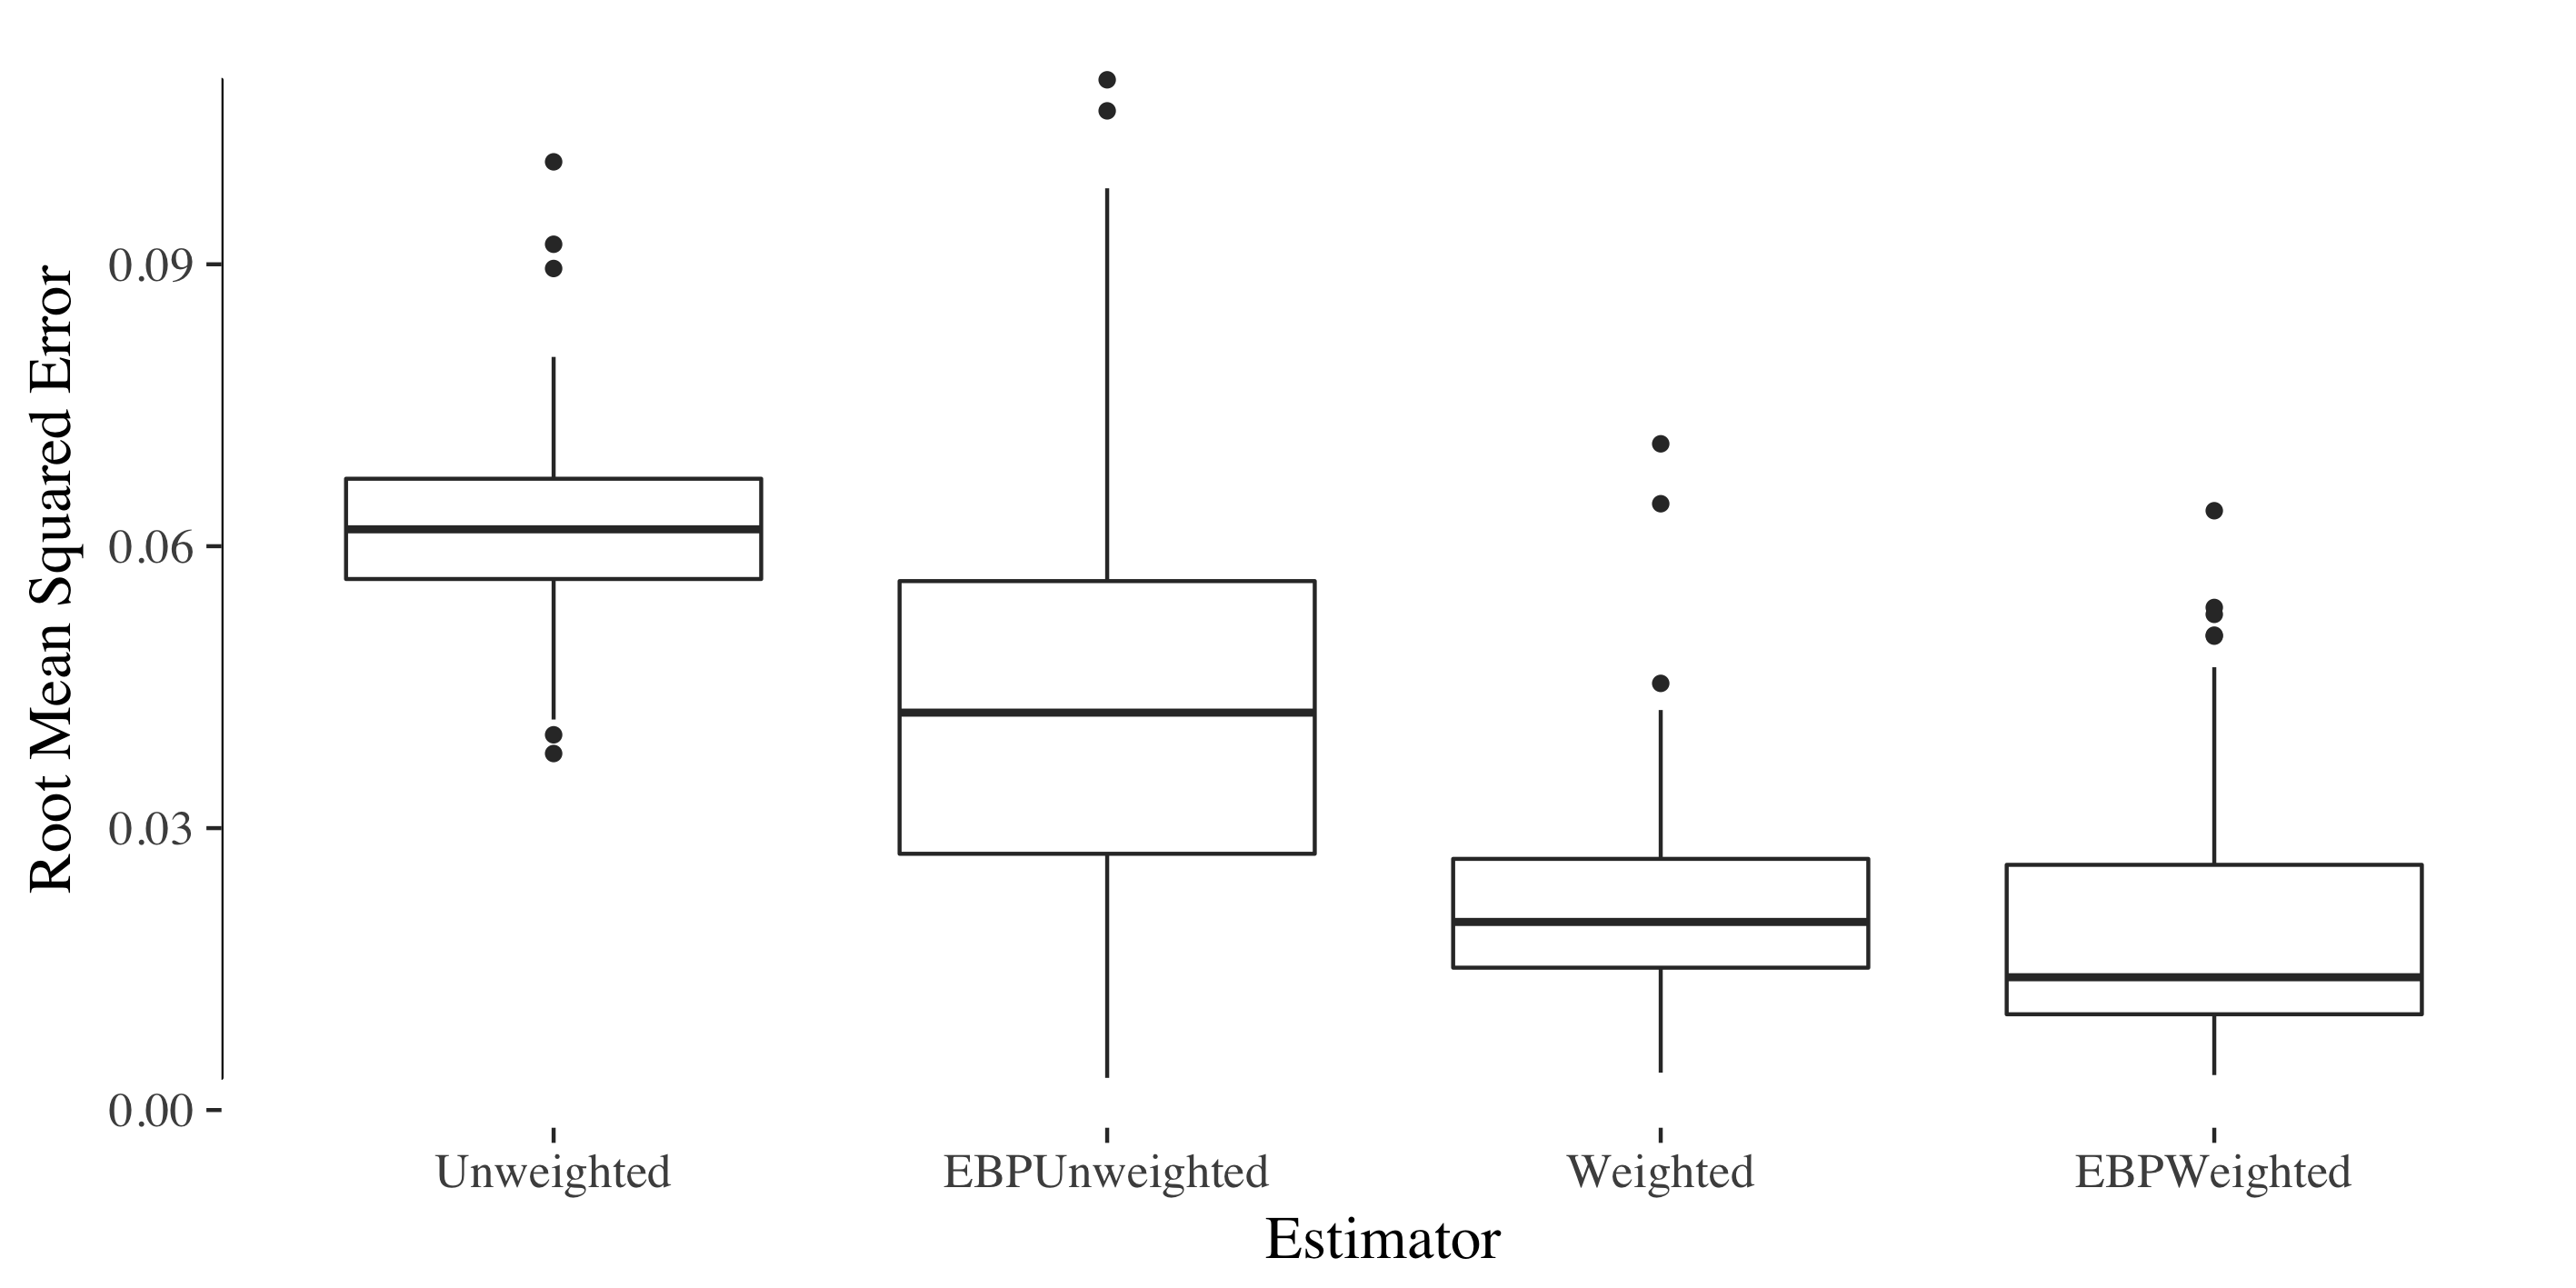
\includegraphics[width=0.9\textwidth]{BoxPlotRMSEByDomain}
		\caption{Boxplot of RMSE on Domain Level}
	\end{figure}
\end{center}
\end{block}

\end{column}

%
%-------------------------------------------------------------------------------------------------------------
% 12

\begin{column}{.3\linewidth}


  \begin{block}{ Accuracy of inbuilt MSE estimator \Pheight}
	\begin{center}
	\begin{figure}
		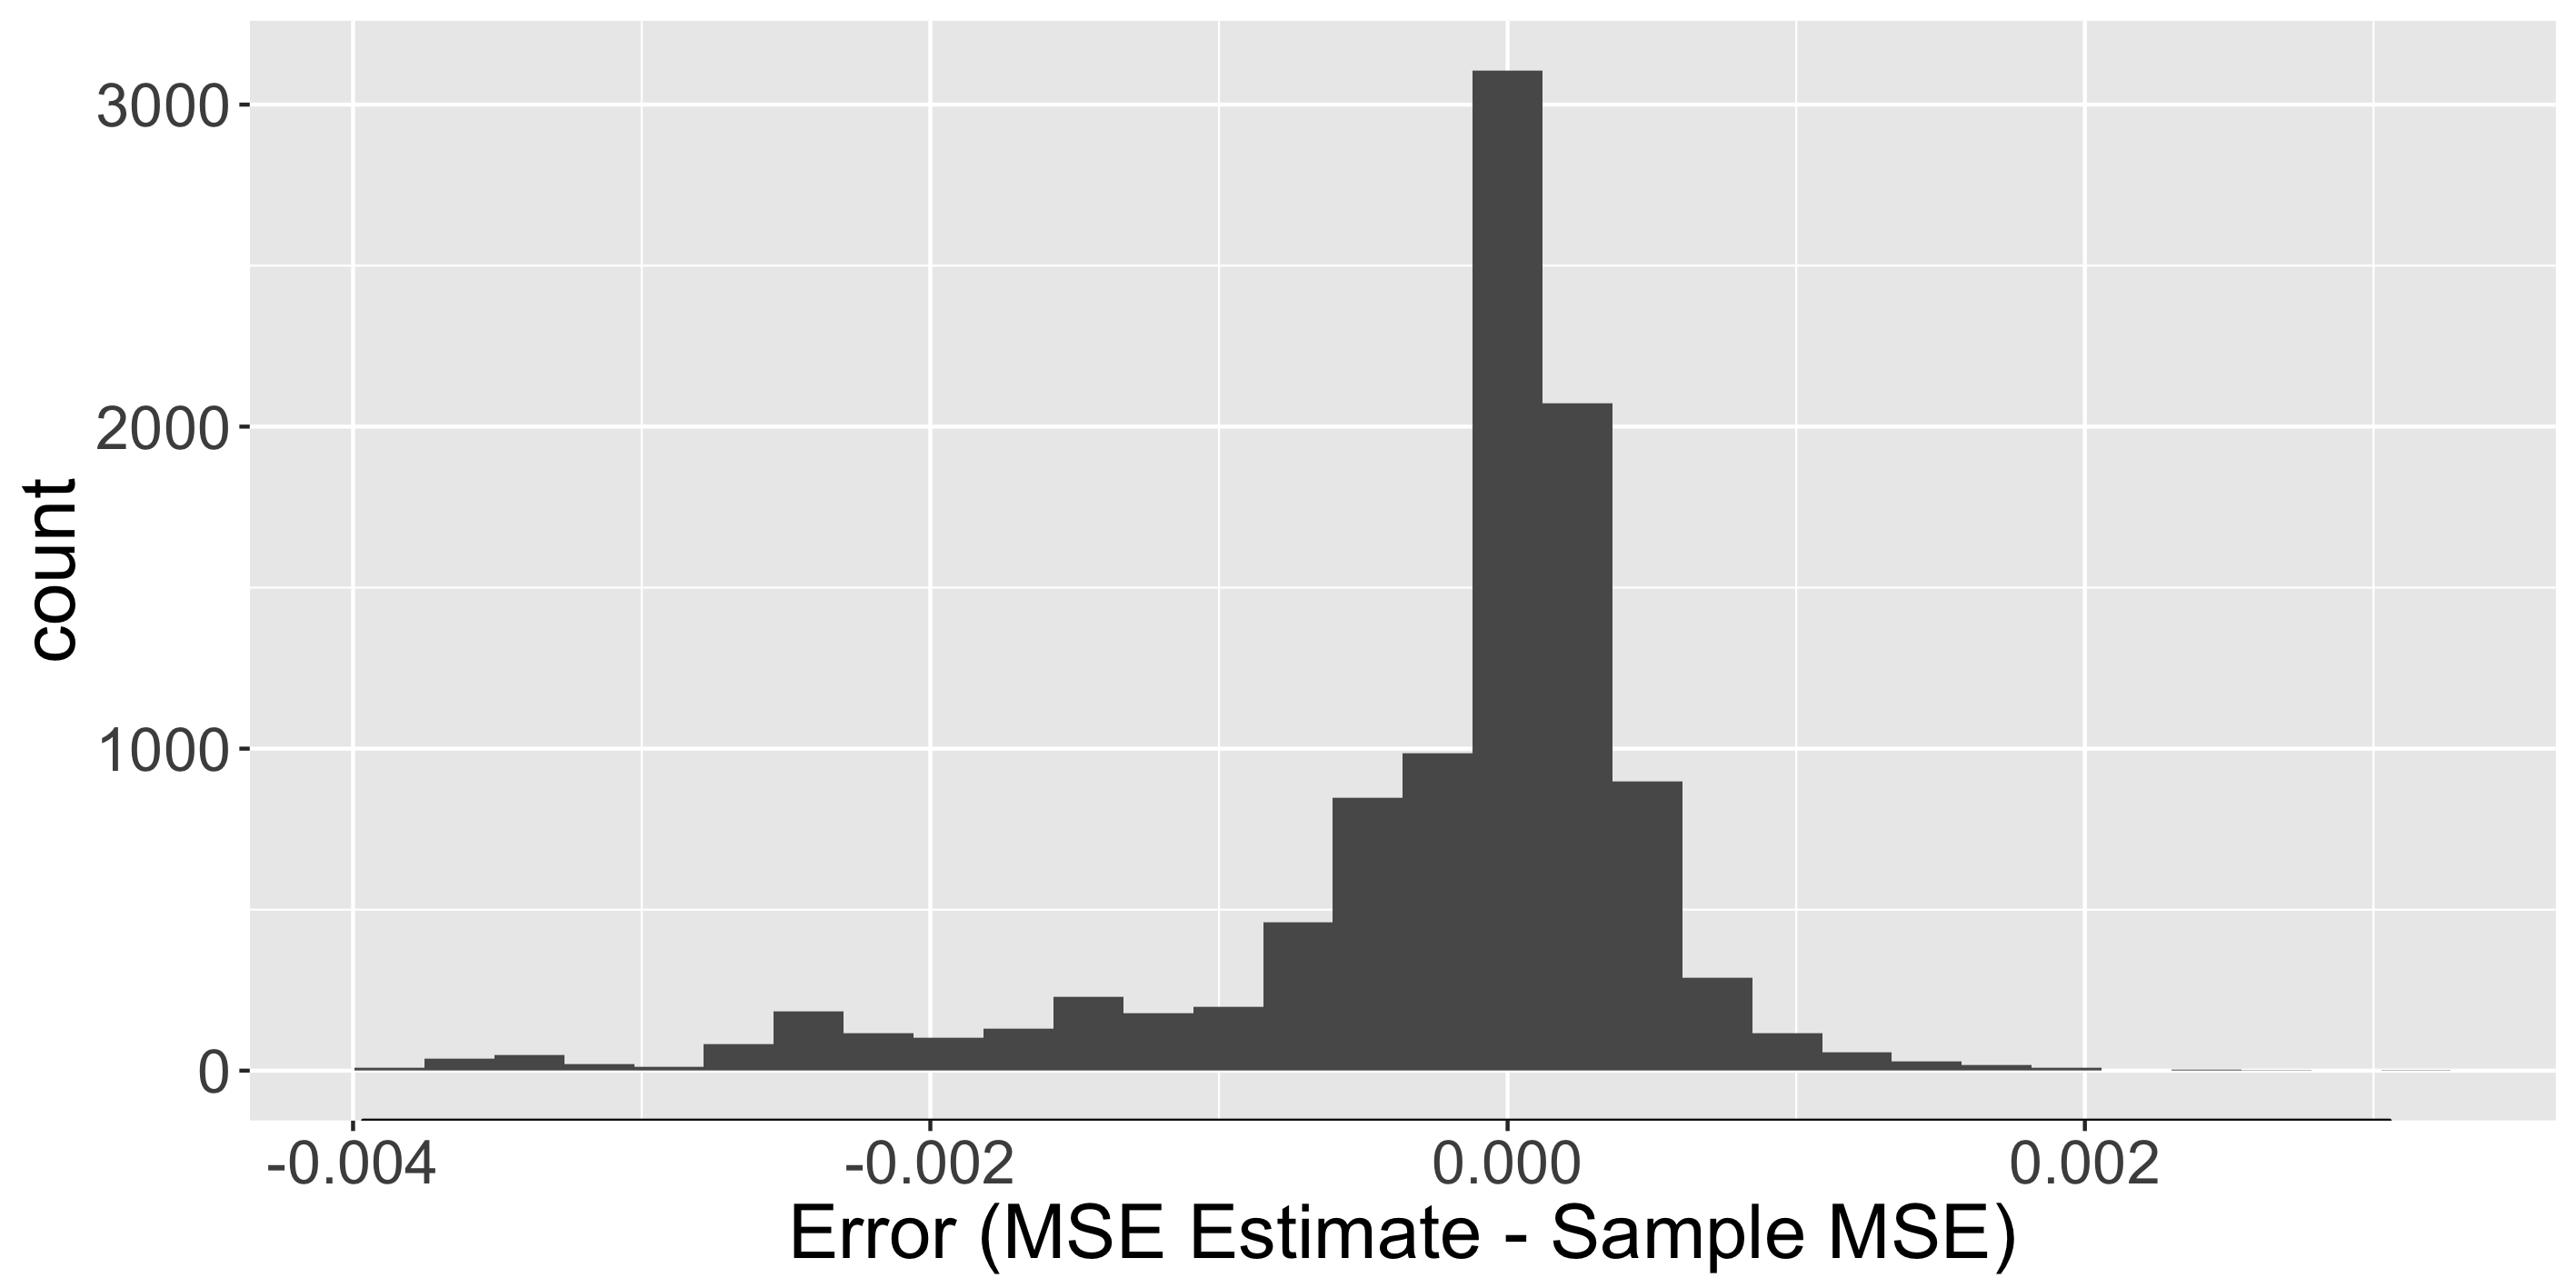
\includegraphics[width=0.9\textwidth]{HistogramMSEEstimate}
		\caption{Histogram of Difference between EBP MSE estimator and the sample MSE across iterations}
	\end{figure}
\end{center}
   \end{block}
\textbf{Observations:}
\begin{itemize}
	\item Bootstrap estimator agrees quite well with sample MSE
	\item Slightly more likely to underestimate sample MSE
\end{itemize}

\end{column}

%
%------------------------------------------------------ ------------------------------------------------------
%

\end{columns}

\end{frame}


\end{document}

